\section{Choix des équipements}

%
%
\subsection{Liaison des bâtiment}

Le nouveau bâtiment est construit à 50 mètres du bâtiment déjà existant,

L'avantage du choix de la fibre optique se porte plus particulièrement sur une connexion optimale offrant un débit bien plus supérieur que l'ADSL,
La fibre optique limite les pertes de signal et accentue son avantage sur le très haut débit, Cependant il faut noter qu'il n'est pas nécessaire de modifier totalement l'infrastructure réseau, Sa vitesse dépend de l'équipement aux extrémités de la fibre, C'est pour cela qu'il est préjudiciable d'opter pour un routeur performant,

Pourquoi mettre une fibre multimode plutôt qu'une fibre monomode ?
La fibre multimode est utilisée pour des courtes distances, En effet, les rayons lumineux qui se propagent peuvent suivre des angles de réfraction différents, Ses performances avoisinent 1Gb/s pour une longueur de 100 mètres, La fibre multimode est plus employée pour des réseaux privés
Tandis que la fibre monomode dispose d'une dispersion du signal quasi nulle et son cœur est plus fin, C'est grâce à ces caractéristiques que ses performances se font ressentir jusqu'à atteindre environs 100 Gb/s, Ce type de fibre est utilisé pour les sites distants, Grâce à son cœur de petit diamètre, la puissance d'émission est plus conséquente, les rayons suivent un seul chemin, Du fait de ses débits très importants, mais de son coût élevé, cette fibre est utilisée essentiellement pour les sites à grande distance et très grande distance,

Concernant le routeur d'extrémité de l'ancien bâtiment, il devrait supporter le débit annoncé de la fibre optique ainsi que sa connectique,
Si malencontreusement cette connective n'existe pas il est possible de prendre un module convertisseur de mode fibre appelé SFP,

Il faudra pour cela se munir de connecteurs SC fibre optique pour sertir les embouts désirés et ensuite les raccorder, Quatre connecteurs suffisent pour relier les 2 fibres,  Nous en rajoutons deux en cas de défaillance,

Le choix de la fibre optique porte sur les critères suivants :
La longueur doit être au moins supérieure à 50m X 2 = 100 mètres, En effet la fibre est doublée pour assurer une redondance d'échanges,
Son débit
Son prix
Nous prennons donc deux bobines de 100m de fibre qu'il sera possible de bien délimiter la distance et le sertir suivant la convenance lors de l'installation,


\subsection{Équipements réseau}

\subsubsection{Routeurs}

Commençons par les deux routeurs du cœur de réseau qui devront prendre en charge des services nécessaires au bon fonctionnement hospitalier :
La première fonction est de transférer les paquets en direction de l'ancien bâtiment afin que le routeur puisse les router jusqu'à internet si besoin,
La seconde fonction est d'assurer les services VOIP et Wifi (des routeurs et des commutateur proposent nativement ces fonctionnalités) redirigés par l'ancien bâtiment
La troisième fonction est de gérer les mêmes services que l'ancien bâtiment : Sauvegarde de fiches patientes, base de données,

\begin{figure}
    \center
    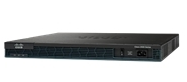
\includegraphics[width=0.5\textwidth]{./images/7.png}
    \caption{Un routeur}
\end{figure}

Les deux routeurs sont redondés pour assurer une pérennité des équipements,
La particularité principale sur la sélection d'un routeur est la fonctionnalité qu'il fasse du Gigabit,
Le SFP est aussi important qui est un module intégré de convertisseur mode fibre, Dans le cas où dans l'ancien bâtiment, il ne dispose pas de cette fonctionnalité pour assurer la fibre optique, il sera préférable de prévoir un achat SFP,

Nous avons sélectionné donc deux routeurs au choix :



    \begin{center}
        \begin{tabular}{|l|p{5cm}|p{5cm}|}
          \hline
            Marque  &   TP-Link : T3700G-28TQ    &   Cisco 2901 \\
          \hline
            Debit  &
Gigabit Ethernet
24 x 10/100/1000 + 4 x SFP Gigabit combiné + 2 x 10 Gigabit SFP
   &   Gigabit Ethernet
10/100/1000
Ethernet, Fast Ethernet, Gigabit Ethernet \\
          \hline

Protocoles supportés
  &   RIP-1, RIP-2, IGMP, VRRP, OSPFv2, PIM-SM, routage IP statique, PIM-DM, ECMP
SNMP 1, RMON 1, RMON 2, RMON 3, RMON 9, SNMP 3, SNMP 2c, HTTP, TFTP, SSH, SSH-2, CLI   &   OSPF, IS-IS, BGP, EIGRP, DVMRP, PIM-SM, IGMPv3, GRE, PIM-SSM, routage statique IPv4, routage statique IPv \\
          \hline
            Performances  &
Capacité de commutation : 128 Gbps
   &
Capacité de commutation : allant 128 Gbps et +
 \\
          \hline
            Tables  &
32 000 entrées
   &
n/c
 \\
          \hline
            Commentaires  &
Conformité aux normes, toutes configurations, controle de flux, DHCP, STP, ACL, VLAN etc,,,
   &
Conformité aux normes, toutes configurations, Cisco IOS Security, controle de flux, DHCP, STP, ACL, VLAN etc,,,
 \\
          \hline
            Dimensions  &
$44 cm * 33 cm * 4,4 cm$
   &
$43,8 cm * 43,9 cm * 4,5 cm$
 \\
          \hline
            Prix
            &
            $1884,11 * 2 = 3768,22  \euro$
            &
            $1909 * 2 = 3818  \euro$
 \\
          \hline
        \end{tabular}
    \end{center}

Une fois les routeurs sélectionnés, le choix des commutateurs avec routage réservés à la distribution, auront pour rôle de répartir chaque trame qui circule dans le réseau, Comme expliqué ci-avant un commutateur avec routage permet d'interconnecter des réseaux homogènes ici dans notre cas : les étages de ce nouveau bâtiment,
Par la suite des commutateur devront être installés au niveau de chaque étage dont un qui est principal qui assure l'ensemble des liens et de la fonctionnalité voix,


\subsubsection{Commutateurs}

Pour continuer, le choix des équipements supplémentaires se portent sur les commutateur qui commuteront des trames, Deux commutateur seront préconisés, En effet redonder un commutateur permet de bien séquencer les trames, éviter les domaines de collisions et assurer la panne matérielle,
Le choix des commutateur se porte principalement sur la capacité à transmettre les trames, Des ports de haut débit permettront d'améliorer le débit de transit reliés au routeur,

\begin{figure}[!ht]
    \center
    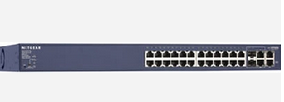
\includegraphics[width=0.5\textwidth]{./images/10.png}
    \caption{Un commutateur}
\end{figure}

Nous prévoyons 2 commutateurs supplémentaires par étage pour assurer la disponibilité,

Nous proposerons 2 commutateurs au choix afin de ne pas se focaliser sur un matériel a proprement dit,
Nous allons structurer le choix des matériels par étage :
A l'étage N-1 : étage critique nous avons  besoin d'un seul commutateur de niveau 2 et 24 ports pour l'ensemble des terminaux,


    \begin{center}
        \begin{tabular}{|l|p{4cm}|p{4cm}|p{4cm}|}
          \hline
            Marque  &  TP-Link TL-SG3424 &   CISCO SF220-24 &  Netgear FS728TPv1 \\
          \hline

Nombre de ports
  &   24 x 10/100 + 2 x combo Gigabit SFP
    &   24 x 10/100 + 2 x combo Gigabit SFP
24 x 10Base-T/100Base-TX - RJ-45
24 x 10Base-T/100Base-TX - RJ-45 - PoE
2 x 10Base-T/100Base-TX/1000Base-T - RJ-45
2 x SFP  & 24 ports Ethernet
4 ports Gigabit
Multicast VLAN Registration \\
          \hline
            Dimensions  &   $440 * 330 * 44 mm $                       &   $440 * 201 * 44 mm$ & $440 * 257 * 44 mm$                 \\
          \hline
            Prix  &
$224,90 \euro   $
    &
$214,90  \euro   $
 &
$269,90  \euro   $
 \\
          \hline
        \end{tabular}
    \end{center}

Pour l'étage N1, il faut 2 commutateur de 24 ports chacun pour raccorder l'ensemble des téléphones IP des postes ainsi que des bornes Wifi,
Revenons au tableau de l'étage N-1 le choix peut se faire suivant les caractéristiques de ces deux matériels choisis,
Chacun d'eux supporte bien évidemment la voix et à des caractéristiques appréciables,
Prenons donc l'hypothèse du choix du commutateur CISCO de 24 ports chacun, pour cela il faut débourser la somme de $214,90 \euro    X 2 = 429,80  \euro$.

Pour les étages N2 à N4 il faut 2 commutateur 24 ports,
Nous gardons l'hypothèse du commutateur CISCO de 214,90  \euro    sachant qu'il en faut deux par étage il en faut donc 6 au total,
Or nous privilégions un surplus en cas de panne majeure et pouvoir les remplacer,
Deux commutateurs supplémentaires semble suffisant,
Un total de $214,90 * 6 + 214,90 * 2 = 2369,20  \euro    $



\subsubsection{Serveur lame }

Un serveur lame est un serveur de petite taille facilitant l'installation de celui-ci dans une armoire de brassage,

\begin{figure}[!ht]
    \center
    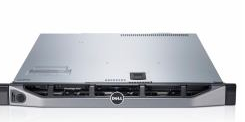
\includegraphics[width=0.5\textwidth]{./images/13.png}
    \caption{Un serveur applicatif}
\end{figure}

L'un des  avantages de ce type de serveur est son coût acquisition,
En effet au fil du temps son retour sur investissement coûte moins cher qu'une exploitation standard de machine serveur,
De plus sa mise en place est bien plus rapide et efficace,

Nous avons sélectionné deux types de serveur, Le choix s'est porté sur leur caractéristiques et sur leur services rendus,

    \begin{center}
        \begin{tabular}{|l|p{5cm}|p{5cm}|}
          \hline
            Marque  &
Power Edge R220 Dell
    &   DELL PowerEdge R320
 \\
          \hline
Processeur
  &
Intel Xeon
    &
Intel Xeon
 \\
          \hline
Mémoire RAM
  &
8 Go
    &
8 Go
 \\
          \hline
            Caractéristiques  &
4000 gigaoctets 7200 RPM en RAID 1, PERC H310, iDRAC7 Express, DVDRW, 2x GLAN, 250W
                & 16 To, technologie de virtualisation, SATA, RAID, alimentation 350 W
6 coeurs
                  \\
        \hline
            Prix  &
$920.05 * 2 = 1840.10 \euro   $
    &
$1544 * 2 = 3088 \euro   $
 \\
          \hline
        \end{tabular}
    \end{center}

Le choix de ces serveurs lame se caractérise par leur extensibilité pour le futur. En effet si le besoin de mémoire se fait ressentir par exemple, alors il sera possible d'agrémenter des ressources dans ces serveurs. De plus ces serveurs ont un prix abordable pour le besoin souhaité. Il est même possible de faire l'acquisition d'un serveur machine mais sa particularité imposante et limitée en ergonomie ne facilitera pas le retour sur investissement à long terme. Il sera donc nécessaire de les changer dans 5-8 ans.


\subsubsection{Serveur NAS}

Un serveur NAS est un équipement à part entière. Il permet de faire du stockage réseau à grande quantité.
Sa particularité est son coût mais aussi sa forte capacité de stockage.

Le NAS permet à l'ensemble de l'équipe hospitalier de sauvegarder périodiquement un ensemble de données modifiées dans la base de données. Cet accès au stockage permet également de consulter les informations d'un patient par exemple.

\begin{figure}[!ht]
    \center
    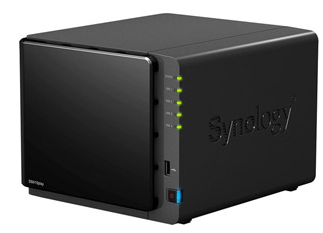
\includegraphics[width=0.5\textwidth]{./images/15.png}
    \caption{Un NAS}
\end{figure}

Nous avons choisi deux NAS aux prix différents. Le choix se fera en fonction du besoin précis de la capacité et au nombre de disques désirés.
Le choix d'un serveur NAS se détermine également par la fonctionnalité du RAID supporté.

RAID 5
le RAID 5 tolère la panne d'un disque dur. Cette particularité du RAID 5 a besoin d'un minimum de 3 disques durs. Contrairement à la copie en miroir, le RAID 5 assure la redondance des informations des disques en stockant les information de parité. Il faut cependant privilégier des disque de même capacité et de même marque si besoin.


    \begin{center}
        \begin{tabular}{|l|p{5cm}|p{5cm}|}
          \hline
            Marque  &
Synology Disk Station DS2415
    &   Synology DiskStation DS415Play
 \\
          \hline
Capacité du NAS
  &
6 disques pour $96To$
    &
4 disque pour $24To$
 \\
          \hline
compatible services réseaux
  &
TCP/ IP, PPTP, PPPoE, iSCS, FTP, NFS, AD webdev, AFP, CalDAV, DHCP, DNS, DDNS, SNMP, Telnet, SSH
    &
TCP/ IP, PPTP, PPPoE, iSCSI, FTP, DHCP, DNS, DDNS, SNMP, Telnet, SSH
 \\
          \hline
            Caractéristiques  &
4000 gigaoctets 7200 RPM en RAID 1, PERC H310, iDRAC7 Express, DVDRW, 2x GLAN, 250W
                & 16 To, technologie de virtualisation, SATA, RAID, alimentation 350 W
6 coeurs
                  \\
        \hline
            Prix avec disques &
$1236 + 139.50 * 12 = 2910 \euro   $
    &
$425 + 226.66 * 4 = 1331.64 \euro   $
 \\
          \hline
        \end{tabular}
    \end{center}


\subsubsection{Onduleur}

Un onduleur est un équipement permettant de sécuriser l'ensemble des équipements inter-connectés. Il s'agit d'un dispositif électronique de forte puissance qui permet de délivrer des tensions et des courants alternatifs à partir d'une source d'énergie électrique continue. De ce fait il préserve l'extinction des équipements.

L'onduleur sélectionné sera branché avec les équipements :
Routeurs
serveurs Lame
NAS

Il nous en faut au moins 5 prises pour les différents équipements.

\begin{figure}[!ht]
    \center
    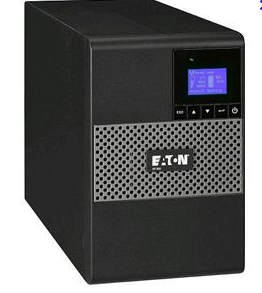
\includegraphics[width=0.4\textwidth]{./images/18.png}
\end{figure}

800 W et comporte 8 prises pour un prix d'environ 300 \euro



\subsubsection{Bornes WiFi}

Concernant les bornes Wi-fi, une borne 2.4Ghz destinée pour les patients est installée sur chaque étage et deux bornes double bande soit 5Ghz destinées pour l'ensemble du personnel pour assurer une continuité d'accès fiable au réseau sans-fil.

\begin{figure}[!ht]
    \center
    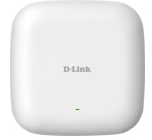
\includegraphics[width=0.5\textwidth]{./images/20.png}
\end{figure}

Un tableau comparatif de bornes Wifi 5 Ghz pour le personnel. Ces bornes sont placées au nombre de deux aux étages :
N0 : Accueil
N1 : Bureaux administratifs
N2 à N4  Chambres des patients
Il faut donc 10 bornes Wi-Fi pour couvrir l'ensemble de ce nouveau bâtiment.



    \begin{center}
        \begin{tabular}{|l|p{5cm}|p{5cm}|}
          \hline
            Marque  & Ubiquiti UniFi AP-Pro UAP-Pro
    &   D-Link DAP-2660
 \\
          \hline
Fréquences supportées
  &
Double radio 2.4 GHz et 5 GHz
    &
Double radio 2.4 GHz et 5 GHz
 \\
          \hline
Protocoles de liaison
  & IEEE 802.11a
IEEE 802.11b
IEEE 802.11g
IEEE 802.11n
    & IEEE 802.11a
IEEE 802.11b
IEEE 802.11g
IEEE 802.11n
 \\
          \hline
            Alimentation  & Compatible PoE & Compatible PoE
                  \\
          \hline
            Nombre de connexions  & $100+$ & $100+$
                  \\
          \hline
            Couverture  & $150m$ & $150m$
                  \\
        \hline
            Prix avec disques &
$221.64 * 10 =2216.4 \euro   $
    &
$298.31 * 10 = 2983.1 \euro   $
 \\
          \hline
        \end{tabular}
    \end{center}

Des bornes Wifi configurées seulement sur la bande 2.4 Ghz servent l'ensemble des visiteurs. Ces bornes sont placées au niveau de chaque étages au nombre d'une borne par étage :
N0 : Accueil;
N2 à N4 : Chambres des patients;
Il en faut quatre bornes Wi-Fi  pour couvrir l'ensemble de ce nouveau bâtiment.



\subsubsection{Baie de brassage}


La question qui se pose : quel est le type de baie de brassage à prendre et à quel nombre ?
Ici chaque équipement du cœur de réseau que nous avons sélectionné pour la solution proposée s'adapte aux baies de brassage de taille standard.
Le choix de sa profondeur est un point essentiel à prendre en compte, il faut cependant savoir aussi que la longueur est importante.

\begin{figure}[!ht]
    \center
    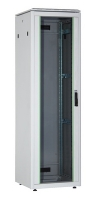
\includegraphics[width=0.3\textwidth]{./images/24.png}
\end{figure}

Il faut donc, cependant prévoir un peu plus large pour l'espace annoncé dans le coeur de réseau. Pour cela, nous prendrons une baie standard de 19 pouces afin que chaque équipement puisse s'intercaler dans chaque compartiments. Nous prenons également une armoire à baie, pour les simples raisons :
Espacement des équipements, facilite l'évacuation de la chaleur
Espace disponible pour de futures installations.
Cette baie sera installée dans le local dédié au coeur de réseau au rez-au-chaussée de l'accueil
Deux baies attirent notre attention pour leur dimension, leur ergonomie, et leur adaptation aux équipements :

    \begin{center}
        \begin{tabular}{|l|p{5cm}|p{5cm}|}
          \hline
            Marque  & LogiLink
    &   DIGITUS
 \\
          \hline
Dimensions
  &
$(L)600 * (P)600 * (H)2.033 mm$
    & $ (L)600 * (P)600 * (H)1.577 mm $

 \\
          \hline
Dimensions tiroirs
  & 19 Pouces standard à tous équipements
    & 19 Pouces standard à tous équipements
 \\
          \hline
            Commentaires   & Porte vitrée, aérations, rehaussement de l'armoire & Porte vitrée, aérations, rehaussement de l'armoire
                  \\
        \hline
            Prix &
$ 578.88 \euro   $
    &
$ 561.13 \euro   $
 \\
          \hline
        \end{tabular}
    \end{center}

Concernant les baies de brassages de chaque niveau, une baies de petite taille suffit car elle accueil seulement deux commutateurs.
Chaque baie sera installée dans un local dédié de chaque étage. Un tableau caractéristique propose deux baies.

\begin{figure}[!ht]
    \center
    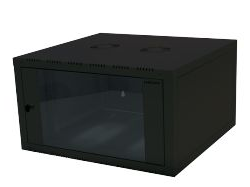
\includegraphics[width=0.5\textwidth]{./images/25.png}
\end{figure}


    \begin{center}
        \begin{tabular}{|l|p{5cm}|p{5cm}|}
          \hline
            Marque  & LogiLink
    &   LogiLink
 \\
          \hline
Dimensions
  &
$(L)600 * (P)560 mm$
    & $ (L)600 * (P)450 mm $

 \\
          \hline
Dimensions tiroirs
  & 19 Pouces
    & 19 Pouces
 \\
          \hline
            Commentaires   & 6U, fixation murale, porte vitrée, aérations & 9U, fixation murale, porte vitrée, aérations
                  \\
        \hline
            Prix &
$ 159.59 * 5 = 797.95  \euro   $
    &
$ 155.03 * 5 = 775.15 \euro   $
 \\
          \hline
        \end{tabular}
    \end{center}





\subsection{Liaison des équipements}

Le choix des câbles n'est pas si facile. En effet plusieurs caractéristiques sont à prendre en compte.

Pour commencer il faut savoir quel type de conducteur est utile.
Le monobrin est constitué de deux fils dont en paire torsadée et une en cuivre massif. Les câbles monobrins peuvent atteindre une portée de 100 mètres et sont destinés à être installés dans des murs ou sous plafond.
Le multibrin est constitué de deux fils également mais d'une paire torsadée mais aussi d'une tresse de micro-fils de cuivre. On les remarque grâce à leur souplesse. Ce type de câble n'est pas similaire au monobrin. En effet le signal est plus atténué. Pour des longueur de moins de 30 mètres il faut les éviter pour éviter ces atténuations.

Le multibrin semble répondre a un environnement professionnel et en gain majeur de transfert.

Il est cependant important de souligner que dans un établissement médical, le type de blindage est à prendre en compte pour en assurer la sécurité. En effet la norme LSZH (Low Smoke Zero Halogene) est obligatoire dans les installations professionnelles dont médicales principalement. Il faut cependant prendre des câbles sans halogène.

Le type de blindage SFTP Shielded Foiled Twisted Pair de Cat6  plus dispose des paires blindées par un écran en aluminium, ainsi la gaine extérieure est aussi blindée par une tresse en cuivre étamé.

Le choix du cable sera donc du cat6a car sa Fréquence inférieur à 500 Mhz et supporte le 10Gbits Ethernet. Ce type de câble permettra d'assurer une certaine évolution si besoin le réseau serait amené à changer.
La catégorie 6 uniquement peut être choisie pour les périphériques finaux  et les étages.

Une longueur raisonnable de 300 mètres de CAT6a devrait couvrir l'ensemble du bâtiment.
Prix : environ $ 268,50 \euro $



\subsection{Climatiseur}

\begin{figure}[!ht]
    \center
    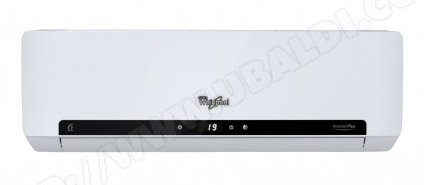
\includegraphics[width=0.4\textwidth]{./images/28.png}
\end{figure}

Garder la pièce du coeur de réseau au frais est important car chaque équipement dégage de la chaleur lors de son fonctionnement. En cas de non respect de la temperature fraiche, des dysfonctionnements d'équipements pourraient survenir. L'ajout d'un climatiseur facilite les équipement à bien fonctionner et à assurer leur activité à long terme.

La température est variable, été comme hiver, ce climatiseur s'adapte à tout type d'environnement.
Cet équipement est important pour assurer une certaine sécurité dans le réseau. Il est évident de dire qu'un réseau bien constitué, peut perdre de ces performances si un climatiseur est inexistant.
Prix : environ $ 601 \euro $



\subsection{Terminaux}

\subsubsection{Ordinateurs}



    \begin{center}
        \begin{tabular}{|l|p{2cm}|p{2cm}|p{2cm}|p{2cm}|}
          \hline
            Caractéristiques  & Ordinateur & Écran & clavier / souris & lecteur de carte vitale \\
          \hline
            Marque  & DELL Ordinateur de bureau Vostro & Philips 18.5" LED - 193V5LSB2 & Dell & Ingenico Xiring \\
        \hline
            Prix &
$ 349 * 21 = 8765.4 \euro   $
    &
$ 85.95 * 21 = 4211.95 \euro   $
    &
$ (14.79 + 18.48) * 21 = 1630.23 \euro   $
    &
$ 229 * 12 = 2748 \euro   $
 \\
          \hline
        \end{tabular}
    \end{center}



\subsubsection{Téléphones}

\begin{figure}[!ht]
    \center
    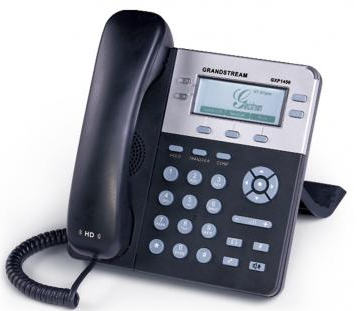
\includegraphics[width=0.4\textwidth]{./images/29.png}
\end{figure}

Les téléphones VOIP fixe destiné aux personnels sont du modèle GXP1450 HD Grandstream.
Ce téléphone à les fonctionnalités suivante: DECT 4 appels simultanés, groupement d'appels, appel entrant, attente, codec vocaux, service sécurisé HTTPS/TFTP/SRTP et dispose d'un écran LCD . Il est raccordable via une interface RJ45 et supporte la technologie PoE. Ils faut 32 téléphones afin de répondre au besoin de la clinique. Le coût unitaire est de 54.43 \euro.

Les téléphones destinés au patients sont eux moins sophistiquer, il n'y a pas d'écrans LCD et ne supporte pas toutes les options cité ci-dessus. Il est aussi raccordé en RJ45 et supporte le PoE.

\begin{figure}[!ht]
    \center
    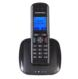
\includegraphics[width=0.2\textwidth]{./images/31.png}
\end{figure}

Pour finir les téléphones sans fil pour le personnel est aussi de la marque GrandStream, et de modèle DP715
Il a les même caractéristique que le téléphones filaire pour le personnel. sont socle doit être à 50 mètres du téléphone.
Son autonomie est de 10h. Le prix unitaire est de 139.95 \euro.


\begin{figure}[!ht]
    \center
    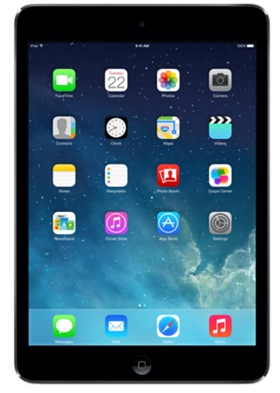
\includegraphics[width=0.3\textwidth]{./images/32.png}
\end{figure}

Les tablettes misent à disposition du personnel sont de la marque Apple et de modèle Ipad Mini. Son autonomie est de 10h et son prix de 300 \euro.




\subsection{Devis}

\begin{itemize}
\item 32 Téléphone VOIP Fixe Personnel (54.43 \euro) : 1741.76\euro ;
\item 60 Téléphone VOIP Fixe Patients (46.90 \euro) : 4221\euro ;
\item   9 packs de 3 Téléphones VOIP sans fil (139.95 \euro )   : 1259.55\euro;
\item  15 Ipad mini 2 Tablette (299 \euro)   : 4489\euro;
\item  28 Ordinateur Médecin (547\euro )   : 18317.936\euro;
\item   21 ordinateur Administratif (349\euro)   : 8765.484\euro;
\item   49 Ecran ordinateur (85.95\euro)   : 4211.55\euro ;
\item   49 Clavier + Souris (33.27\euro)   : 1630.23\euro;
\item  12 Outil carte vitale (229\euro)   : 2748\euro;
\item   300m de Fibre Optique : 369,42 \euro ;
\item  6 + 6 Connecteurs Fibre Optique SFP + SC (22.24 \euro + 6.02 \euro)   : 339.12\euro;
\item     2  Routeur TP-Link : T3700G-28TQ      (1884.11\euro)            :    3768.22\euro    ;
\item       2  Serveur lame Power Edge R220 Dell    (920.05 \euro)            :   1840.10\euro     ;
\item      NAS 48 To avec 12 disques   (1236 \euro + 1674 \euro)            :    2910\euro     ;
\item        Onduleur               :       309.60 \euro  ;
\item          15 Switch Cisco 24p        (214,90 \euro)   :    3223.5\euro     ;
\item              Etage N0 Switch Netgear FS728TPv1 24p       :    269.90\euro     ;
\item        10   kit de mise en rack  (10\euro)            :     100\euro    ;
\item         20  D-Link DAP-2660 (298,31 \euro)            :     5966.2 \euro    ;
\item          Baie de brassage coeur de réseau Logilink          :      578.88 \euro   ;
\item          5 Baie de brassage Etage  (159.59 \euro)            :     797.95\euro    ;
\item            Cable CAT6a 300m          :      216,00\euro   ;
\item            Climatiseur coeur de réseau          :     601\euro    .
\end{itemize}

Le prix annoncé de 67991.45\euro  rassemble donc tous les critères de configurations explicité dans ce document.



%
